\chapter[Sprint 2 : Salle d'entretien temps réel]{Sprint 2 : Une salle d'entretien temps réel\\et la planification des sessions}
\begin{spacing}{1.2}
\minitoc%
\thispagestyle{MyStyle}
\end{spacing}
\clearpage

\providecommand{\screenshot}[2]{%
  \IfFileExists{../screenshoot/#1}{%
    \includegraphics[width=0.9\textwidth,height=12cm,keepaspectratio]{../screenshoot/#1}%
  }{%
    \fbox{\parbox[c][4.5cm][c]{0.9\textwidth}{\centering\itshape
      Capture d'écran à insérer~: #2\\[4pt]
      \normalfont\small(fichier attendu~: \texttt{screenshoot/#1})}}%
  }%
}

\section{Introduction}

Ce chapitre détaille le Sprint~2, consacré à la dimension temps réel de la plateforme NextHire. Il couvre l'ensemble du parcours qui conduit un candidat présélectionné jusqu'à un entretien en direct~: la planification de la rencontre, la création et la jonction d'une salle d'entretien sécurisée, puis l'établissement d'une communication audio et vidéo synchrone entre le candidat et le recruteur. Le chapitre présente successivement les objectifs et le backlog du sprint, le concept de la salle d'entretien synchrone, sa conception détaillée illustrée par des diagrammes de séquence, puis les interfaces réalisées.

\section{Objectifs du sprint}

L'objectif principal de ce sprint est défini comme suit~:

\begin{quote}
\itshape Doter NextHire d'un canal d'entretien synchrone~: permettre à un candidat de planifier son entretien, de rejoindre une salle d'entretien sécurisée et d'y dialoguer en direct avec le recruteur, grâce à une communication temps réel fondée sur WebRTC et Socket.IO.
\end{quote}

\subsection{Backlog du sprint}

Pour atteindre cet objectif, un sous-ensemble du \textit{product backlog} a été sélectionné puis affiné en récits utilisateurs et tâches techniques, afin de constituer le backlog du Sprint~2 (tableau~\ref{tab:backlog-s2}). Comme pour le \textit{product backlog}, chaque élément est priorisé selon la méthode \textbf{MoSCoW} (\textbf{Must}, \textbf{Should}, \textbf{Could}) et estimé en \textit{story points} sur la suite de Fibonacci (1, 2, 3, 5, 8, 13), soit un engagement de 46~points pour ce sprint.

\begin{table}[H]
  \centering
  \footnotesize
  \renewcommand{\arraystretch}{1.3}
  \setlength{\tabcolsep}{5pt}
  \begin{tabularx}{\textwidth}{|>{\centering\arraybackslash}p{1.1cm}|>{\raggedright\arraybackslash}X|>{\centering\arraybackslash}p{1.7cm}|>{\centering\arraybackslash}p{0.9cm}|}
    \hline
    \rowcolor{blue!10}
    \textbf{ID} & \textbf{Récit utilisateur / tâche} & \textbf{Priorité} & \textbf{Est.} \\
    \hline
    T-02 & Mettre en place le micro-service de planification (FastAPI) intégré au calendrier Google (OAuth~2.0) et à l'envoi de courriels de confirmation. & Must & 8 \\
    \hline
    T-03 & Établir l'infrastructure de communication temps réel~: serveur de signalisation Socket.IO et échange de flux audio/vidéo WebRTC. & Must & 8 \\
    \hline
    S1 & En tant que recruteur, je veux lancer la planification et proposer au candidat des créneaux issus de mon calendrier Google. & Must & 5 \\
    \hline
    S2 & En tant que candidat, je veux choisir l'un des créneaux proposés afin de confirmer mon entretien, avec notification automatique par courriel. & Must & 3 \\
    \hline
    S3 & En tant que recruteur, je veux créer une salle d'entretien partageable associée à un poste et à un candidat. & Must & 3 \\
    \hline
    S4 & En tant que candidat, je veux consulter en temps réel les salles d'entretien disponibles et demander à en rejoindre une. & Must & 5 \\
    \hline
    S5 & En tant que recruteur, je veux admettre le candidat dans la salle et démarrer la session d'entretien en direct. & Must & 3 \\
    \hline
    S6 & En tant que participant, je veux dialoguer en audio et vidéo en direct dans la salle, les changements d'état de la session étant diffusés en temps réel à tous les participants. & Must & 8 \\
    \hline
    T-04 & Améliorer les interfaces des espaces candidat et recruteur (planification, liste des salles, salle d'entretien en direct). & Should & 3 \\
    \hline
  \end{tabularx}
  \caption{Backlog du Sprint~2 : planification et salle d'entretien temps réel.}
  \label{tab:backlog-s2}
\end{table}

\section{Concept de la salle d'entretien synchrone}

\subsection{De l'entretien asynchrone à l'entretien synchrone}

La plupart des plateformes de recrutement assisté par l'IA reposent sur l'entretien vidéo \textit{asynchrone}~: le candidat répond seul, face à son écran, à des questions préenregistrées. NextHire fait le choix inverse d'un entretien \textit{synchrone}, conduit en direct dans une salle partagée. Cette salle réunit le candidat et le recruteur (puis, au sprint suivant, l'agent d'entretien vocal) au sein d'une même session, où chaque action (question, réponse, transcription, changement d'état) est diffusée à tous les participants en temps réel. Ce parti pris rend l'échange plus humain et permet une évaluation adaptative, mais impose une infrastructure temps réel robuste, objet de ce sprint.

\subsection{Cycle de vie d'une session d'entretien}

Chaque session est matérialisée par une entité \texttt{CallRoom} qui suit un cycle de vie clair, piloté par deux rôles~:

\begin{itemize}
  \item \textbf{L'hôte (recruteur)} crée la salle pour un poste et un candidat donnés, puis admet le candidat et démarre la session.
  \item \textbf{Le participant (candidat)} découvre la salle dans la liste des salles disponibles, demande à la rejoindre, puis y accède une fois admis.
\end{itemize}

La salle traverse trois états successifs~: \textbf{en attente} (\textit{waiting}, salle créée mais candidat non encore admis), \textbf{active} (entretien en cours) et \textbf{terminée} (\textit{ended}). Chaque transition est diffusée en temps réel à l'ensemble des participants via Socket.IO.

\section{Conception détaillée et architecture}

La conception de ce sprint s'appuie sur les trois protocoles complémentaires présentés au chapitre~\ref{ch:sprint0} (Sprint~0)~: REST pour les opérations CRUD, Socket.IO pour la signalisation et les échanges en temps réel, et WebRTC pour les flux audio et vidéo pair-à-pair. Les trois sections suivantes détaillent les principaux flux, planification, création et jonction de la salle, établissement de la connexion temps réel, chacun illustré par un diagramme de séquence.

\subsection{Planification des entretiens}

La planification est assurée par un micro-service Python (FastAPI, port~5004) dédié. À partir des disponibilités du recruteur, lues dans son calendrier Google, le service \textbf{génère et classe des créneaux proposés}, puis transmet au candidat un lien de confirmation par courriel. Lorsque le candidat retient l'un de ces créneaux, le service crée l'événement correspondant dans Google Calendar (API OAuth~2.0), notifie les deux parties, puis avertit le BFF Node.js par une route interne. La figure~\ref{fig:seq-scheduling} illustre ce flux.

\begin{figure}[H]
  \centering
  \resizebox{\textwidth}{!}{%
  \begin{tikzpicture}[
    font=\scriptsize, >={Stealth[length=2mm]},
    msg/.style={->, thin},
    ret/.style={->, thin, dashed},
    lbl/.style={font=\tiny, fill=white, inner sep=1pt, midway, above},
    lifeline/.style={dashed, thin, gray!70},
    phdr/.style={draw, fill=blue!12, rounded corners=2pt, align=center,
                 font=\scriptsize\bfseries, minimum height=0.7cm, minimum width=2.6cm},
  ]
    \node[phdr] at ( 0,0) {Recruteur\\(React)};
    \node[phdr] at ( 5,0) {Node BFF\\(:3001)};
    \node[phdr] at (10,0) {Scheduling\\(:5004)};
    \node[phdr] at (15,0) {Google Calendar\\+ SMTP};
    \node[phdr] at (19.5,0) {Candidat\\(courriel/React)};
    \foreach \x in {0,5,10,15,19.5}{ \draw[lifeline] (\x,-0.42) -- (\x,-9.8); }

    \draw[msg] ( 0,-0.85) -- node[lbl] {lancer la planification \{candidat, poste\}} (5,-0.85);
    \draw[msg] ( 5,-1.55) -- node[lbl] {POST /api/scheduling/start} (10,-1.55);
    \draw[msg] (10,-2.25) -- node[lbl] {lire les disponibilités du recruteur} (15,-2.25);
    \draw[ret] (15,-2.95) -- node[lbl] {\{créneaux occupés\}} (10,-2.95);
    \draw[->] (10,-3.45) -- ++(0.55,0) -- ++(0,-0.4) -- ++(-0.55,0);
    \node[font=\tiny, anchor=west] at (10.65,-3.65) {générer et classer les créneaux proposés};
    \draw[msg] (10,-4.35) -- node[lbl] {courriel : lien de confirmation} (19.5,-4.35);

    \draw[draw=gray!55, fill=gray!8, rounded corners=2pt, thin] (8.5,-4.8) rectangle (19.0,-5.25);
    \node[font=\tiny, anchor=west] at (8.6,-5.02) {Le candidat ouvre le lien et choisit un créneau};

    \draw[msg] (19.5,-5.65) -- node[lbl] {GET /api/scheduling/public/\{token\}} (10,-5.65);
    \draw[ret] (10,-6.35) -- node[lbl] {\{créneaux proposés\}} (19.5,-6.35);
    \draw[msg] (19.5,-7.05) -- node[lbl] {POST /api/scheduling/public/\{token\}/confirm} (10,-7.05);
    \draw[msg] (10,-7.75) -- node[lbl] {créer l'événement} (15,-7.75);
    \draw[ret] (15,-8.45) -- node[lbl] {\{eventLink\}} (10,-8.45);
    \draw[msg] (10,-9.15) -- node[lbl] {notifier les deux parties (courriels)} (15,-9.15);
    \draw[ret] (10,-9.65) -- node[lbl] {callback /internal/scheduling/candidate-confirmation} (5,-9.65);
  \end{tikzpicture}}
  \caption{Diagramme de séquence : planification d'un entretien (créneaux proposés au candidat).}
  \label{fig:seq-scheduling}
\end{figure}

\subsection{Création et jonction d'une salle d'entretien}

Le cycle de vie d'une session est piloté par le routeur \texttt{callRoom} en coordination avec \texttt{interviewRoute}. Le recruteur crée une salle, qui apparaît instantanément dans la liste des salles disponibles des candidats concernés~; le candidat demande à la rejoindre, et le recruteur confirme son admission. Les principaux points de terminaison sont~:

\begin{itemize}
  \item \texttt{POST /api/call-rooms/create} crée une nouvelle salle d'entretien pour un candidat et un poste donnés.
  \item \texttt{GET /api/call-rooms/available} retourne la liste des salles d'entretien ouvertes pour le candidat.
  \item \texttt{GET /api/call-rooms/:roomId} retourne le contexte complet de la session (profil candidat, exigences du poste, statut).
\end{itemize}

\noindent La signalisation temps réel s'appuie sur les événements Socket.IO émis par les clients (\texttt{call-\allowbreak room-\allowbreak created}, \texttt{call-\allowbreak room-\allowbreak join-\allowbreak request}, \texttt{confirm-\allowbreak candidate-\allowbreak join}), que le serveur relaie sous des noms dédiés (\texttt{new-\allowbreak call-\allowbreak room}, \texttt{candidate-\allowbreak join-\allowbreak request}, \texttt{join-\allowbreak confirmed}), ainsi que sur \texttt{call-\allowbreak room-\allowbreak status-\allowbreak update} pour la mise à jour de la liste des salles disponibles. La figure~\ref{fig:seq-room} en présente l'enchaînement.

\begin{figure}[H]
  \centering
  \resizebox{\textwidth}{!}{%
  \begin{tikzpicture}[
    font=\scriptsize, >={Stealth[length=2mm]},
    msg/.style={->, thin},
    ret/.style={->, thin, dashed},
    lbl/.style={font=\tiny, fill=white, inner sep=1pt, midway, above},
    lifeline/.style={dashed, thin, gray!70},
    phdr/.style={draw, fill=blue!12, rounded corners=2pt, align=center,
                 font=\scriptsize\bfseries, minimum height=0.7cm, minimum width=3.0cm},
  ]
    \node[phdr] at ( 0,0) {Recruteur\\(React)};
    \node[phdr] at ( 6,0) {Node BFF\\Socket.IO :3001};
    \node[phdr] at (11,0) {MongoDB};
    \node[phdr] at (16,0) {Candidat\\(React)};
    \foreach \x in {0,6,11,16}{ \draw[lifeline] (\x,-0.42) -- (\x,-8.6); }

    \draw[msg] ( 0,-0.85) -- node[lbl] {POST /call-rooms/create \{jobId, candidateId\}} (6,-0.85);
    \draw[msg] ( 6,-1.55) -- node[lbl] {insert CallRoom \{status: waiting\}} (11,-1.55);
    \draw[ret] (11,-2.25) -- node[lbl] {\{roomId\}} (6,-2.25);
    \draw[ret] ( 6,-2.95) -- node[lbl] {\{roomId, status: waiting\}} (0,-2.95);
    \draw[msg] ( 6,-3.65) -- node[lbl] {emit "call-room-created"} (16,-3.65);
    \draw[ret] ( 6,-4.0) -- node[lbl, font=\tiny] {relayé "new-call-room"} (16,-4.0);
    \draw[msg] (16,-4.65) -- node[lbl] {emit "call-room-join-request" \{roomId\}} (6,-4.65);
    \draw[msg] ( 6,-5.35) -- node[lbl] {relayé "candidate-join-request"} (0,-5.35);
    \draw[msg] ( 0,-6.05) -- node[lbl] {emit "confirm-candidate-join"} (6,-6.05);
    \draw[msg] ( 6,-6.75) -- node[lbl] {update CallRoom \{status: active\}} (11,-6.75);
    \draw[ret] ( 6,-7.45) -- node[lbl] {relayé "join-confirmed" $\rightarrow$ redirection} (16,-7.45);
    \draw[ret] ( 6,-8.15) -- node[lbl] {emit "call-room-status-update" \{active\}} (0,-8.15);
  \end{tikzpicture}}
  \caption{Diagramme de séquence : création et jonction d'une salle d'entretien.}
  \label{fig:seq-room}
\end{figure}

\subsection{Signalisation temps réel et établissement WebRTC}

Une fois le candidat admis, la connexion média est négociée par échange de signalisation via Socket.IO~: les deux pairs s'échangent leurs descriptions de session (offre et réponse SDP) puis leurs candidats ICE, le serveur Node se limitant à relayer ces messages entre les deux clients sans jamais y accéder. Une fois la négociation terminée, le flux audio et vidéo circule directement en pair-à-pair entre le candidat et le recruteur, sans transiter par le serveur. La figure~\ref{fig:seq-webrtc} détaille cet établissement.

\begin{figure}[H]
  \centering
  \resizebox{0.92\textwidth}{!}{%
  \begin{tikzpicture}[
    font=\scriptsize, >={Stealth[length=2mm]},
    msg/.style={->, thin},
    ret/.style={->, thin, dashed},
    lbl/.style={font=\tiny, fill=white, inner sep=1pt, midway, above},
    lifeline/.style={dashed, thin, gray!70},
    phdr/.style={draw, fill=blue!12, rounded corners=2pt, align=center,
                 font=\scriptsize\bfseries, minimum height=0.7cm, minimum width=3.0cm},
  ]
    \node[phdr] at ( 0,0) {Candidat\\(React)};
    \node[phdr] at ( 7,0) {Node\\Socket.IO :3001};
    \node[phdr] at (14,0) {Recruteur\\(React)};
    \foreach \x in {0,7,14}{ \draw[lifeline] (\x,-0.42) -- (\x,-9.4); }

    \draw[msg] ( 0,-0.85) -- node[lbl] {emit "join-interview" \{interviewId\}} (7,-0.85);
    \draw[msg] ( 7,-1.55) -- node[lbl] {emit "user-connected"} (14,-1.55);
    \draw[msg] (14,-2.25) -- node[lbl] {emit "offer" \{SDP\}} (7,-2.25);
    \draw[msg] ( 7,-2.95) -- node[lbl] {relais "offer" \{SDP\}} (0,-2.95);
    \draw[msg] ( 0,-3.65) -- node[lbl] {emit "answer" \{SDP\}} (7,-3.65);
    \draw[msg] ( 7,-4.35) -- node[lbl] {relais "answer" \{SDP\}} (14,-4.35);

    \draw[draw=green!50!black, fill=green!5, rounded corners=3pt, dashed, thin]
      (-0.4,-4.8) rectangle (14.4,-6.5);
    \node[font=\tiny\bfseries, text=green!40!black, anchor=north west] at (-0.3,-4.85)
      {loop [échange des candidats ICE]};
    \draw[msg] ( 0,-5.55) -- node[lbl] {emit "ice-candidate"} (7,-5.55);
    \draw[msg] ( 7,-6.15) -- node[lbl] {relais "ice-candidate"} (14,-6.15);

    \draw[<->, very thick, green!45!black] (0,-7.1) -- node[font=\tiny, fill=white, midway]
      {Connexion P2P établie : flux audio/vidéo (WebRTC)} (14,-7.1);
    \draw[msg] ( 7,-8.0) -- node[lbl] {diffusion de l'état de la salle (Socket.IO)} (0,-8.0);
    \draw[msg] ( 7,-8.7) -- node[lbl] {diffusion de l'état de la salle (Socket.IO)} (14,-8.7);
  \end{tikzpicture}}
  \caption{Diagramme de séquence : signalisation et établissement de la connexion WebRTC.}
  \label{fig:seq-webrtc}
\end{figure}

\section{Réalisation et interfaces utilisateur}

Cette section présente les interfaces réalisées au cours du sprint, en suivant le parcours d'un entretien~: planification, création de la salle, accès du candidat, puis entretien en direct.

\subsection{Planification de l'entretien}

Côté recruteur, l'interface de planification permet de lancer la planification et de proposer au candidat des créneaux issus de son calendrier Google (figure~\ref{fig:scheduling-ui}). Le candidat retient ensuite l'un des créneaux depuis le lien reçu par courriel~; sa confirmation déclenche la création de l'événement Google Calendar et l'envoi des courriels de notification aux deux parties.

\begin{figure}[H]
  \centering
  \screenshot{scheduling.JPG}{Planification : proposition et confirmation d'un créneau}
  \caption{Interface de planification d'un entretien côté recruteur.}
  \label{fig:scheduling-ui}
\end{figure}

\subsection{Création de la salle d'entretien}

Le recruteur crée une salle d'entretien associée à un poste~; cette opération génère la session \texttt{CallRoom} partagée et la rend visible aux candidats concernés. Avant le démarrage, les participants se retrouvent dans une salle d'attente (\textit{lobby}), où le recruteur admet le candidat (figure~\ref{fig:room-creation}).

\begin{figure}[H]
  \centering
  \screenshot{room-creation.JPG}{Création d'une salle d'entretien et salle d'attente}
  \caption{Création d'une salle d'entretien et salle d'attente (\textit{lobby}).}
  \label{fig:room-creation}
\end{figure}

\subsection{Salles d'entretien disponibles}

Le candidat dispose d'un écran listant les salles d'entretien disponibles auxquelles il peut se joindre (figure~\ref{fig:available-rooms}), alimenté par la route \texttt{GET /api/call-rooms/available}. Cette liste se met à jour en temps réel grâce à Socket.IO~: lorsqu'un recruteur ouvre une nouvelle salle, celle-ci apparaît instantanément chez les candidats concernés, et toute salle clôturée ou déjà démarrée en est retirée automatiquement. Pour rejoindre un entretien, le candidat envoie une demande (\texttt{call-room-join-request}) puis attend la confirmation du recruteur~; dès que celle-ci est reçue, il est redirigé automatiquement vers la salle. Un mécanisme de secours par interrogation périodique assure cette redirection même si l'événement temps réel venait à être manqué.

\begin{figure}[H]
  \centering
  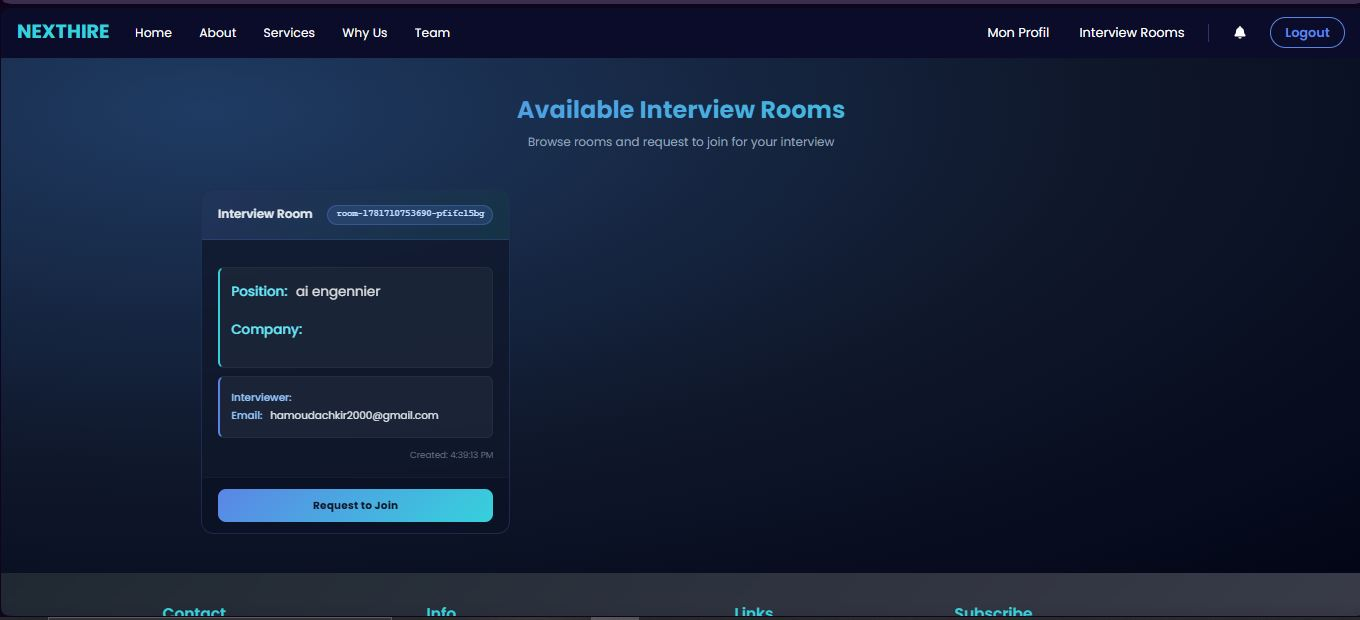
\includegraphics[width=0.9\textwidth,keepaspectratio]{images/available-room.JPG}
  \caption{Liste des salles d'entretien disponibles pour le candidat.}
  \label{fig:available-rooms}
\end{figure}

\subsection{La salle d'entretien en direct}

Une fois le candidat admis, les deux participants se retrouvent dans la salle d'entretien en direct. Les flux audio et vidéo circulent en pair-à-pair grâce à WebRTC, tandis que l'état de la salle et les échanges sont synchronisés en temps réel via Socket.IO (figure~\ref{fig:callroom}). Le pipeline vocal et l'agent d'entretien adaptatif y seront intégrés au sprint suivant.

\begin{figure}[H]
  \centering
  \screenshot{callroom.JPG}{Salle d'entretien temps réel (audio/vidéo WebRTC)}
  \caption{La salle d'entretien en direct entre le candidat et le recruteur.}
  \label{fig:callroom}
\end{figure}

\section{Tests}

La validation de ce sprint a porté sur l'intégration du module de planification (création d'événements Google Calendar et envoi des courriels de confirmation) et sur la signalisation WebRTC/Socket.IO de la salle d'entretien, vérifiée manuellement avec deux clients connectés simultanément (un candidat, un recruteur)~: création de la salle, demande et confirmation de jonction, puis établissement de la connexion audio/vidéo. Les tests automatisés de bout en bout du parcours recruteur sont présentés au chapitre~\ref{ch:sprint5} (Sprint~5).

\section{Conclusion}

Ce sprint a doté NextHire d'un canal d'entretien synchrone complet~: planification intégrée au calendrier, création et jonction d'une salle d'entretien sécurisée, et établissement d'une communication audio et vidéo temps réel entre le candidat et le recruteur. La revue de sprint a permis de dérouler le parcours complet, de la planification jusqu'à la salle en direct, devant nos encadrantes~; la rétrospective a souligné le coût de mise au point de la signalisation WebRTC (traversée NAT, permissions médias), d'où la décision de tester systématiquement les fonctionnalités temps réel sur plusieurs navigateurs et conditions réseau dès les sprints suivants. Le sprint suivant exploite cette salle pour y faire intervenir l'agent d'entretien vocal adaptatif, cœur fonctionnel de la plateforme.
